\documentclass[dvipsnames]{article}
\usepackage{pgfplots}
\usetikzlibrary{decorations.markings}
\pgfplotsset{compat=newest}

% \def\Point{36.9}

\begin{document}

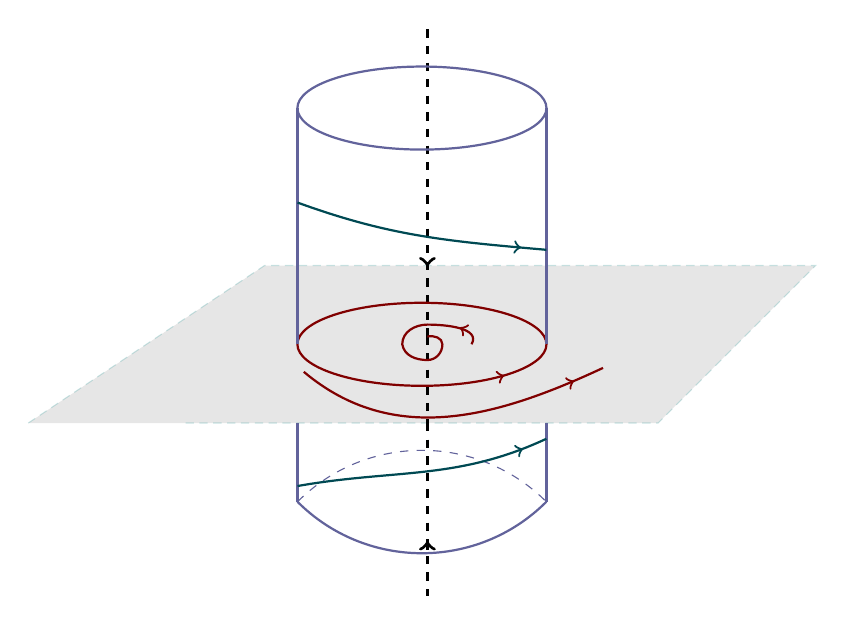
\begin{tikzpicture}
%правая
  % \begin{axis}[
  %   view={-50}{-10}, %угол обзора
  %   axis lines=none,
  %   zmax=60,
  %   height=10cm,
  %   xtick=\empty,
  %   ytick=\empty,
  %   ztick=\empty
  %   ]  
  %   \addplot3+[,ytick=\empty,yticklabel=\empty,
  %   mark=none,
  %   very thick,
  %   color={rgb,255:red,128; green,0; blue,0},
  %   domain=6*pi:10*pi,
  %   postaction={decorate,
  %               decoration={markings,mark=at position 0.9 with {\arrow{<}}}
  %              },
  %   samples=400,
  %   samples y=0,
  %   ]
  %   (-{x*sin(0.17*pi*deg(x))},{x*cos(0.17*pi*deg(x)},{0});
  %   ]
  % \end{axis}
  \draw[teal,densely dashed][fill = gray, opacity=0.2]  (0,3) -- (3,5) -- (10,5) -- (8,3) -- (2,3);
  \draw[very thick] [->] (5.07,5) --(5.07,4.99);
  \draw[very thick, dashed] (5.07,8) --(5.07,4.1);
  \draw[very thick, dashed] (5.07,4.1) --(5.07,3);
  \draw[very thick, dashed] (5.07,3) --(5.07,0.8);
  \draw[very thick] [->] (5.07,1.39) --(5.07,1.5);
  \draw[color={rgb,255:red,128; green,0; blue,0},
      postaction={decorate,
                 decoration={markings,mark=at position 0.9 with {\arrow{>}}}
                }, thick] (3.5,3.65) to [out=-40,in=-155] (7.3,3.7);
  \draw[color={rgb,255:red,128; green,0; blue,0},
      postaction={decorate,
                 decoration={markings,mark=at position 0.9 with {\arrow{>}}}
                }, thick] (5,4) ellipse (45pt and 15pt);
  \draw[color={rgb,255:red,128; green,0; blue,0},
      postaction={decorate,
                 decoration={markings,mark=at position 0.9 with {\arrow{<}}}
                }, thick] (5.07,4.1) to [out=10,in=90] (5.26,4) to [out=-90,in=0] (5.07,3.8) to [out=180,in=-80] (4.75,4) to [out=90,in=180] (5.07,4.25) to [out=0,in=60] (5.63,4);  
\draw[color={rgb,255:red,98; green,99; blue,155},very thick] (3.42,4) -- (3.42,7);
\draw[color={rgb,255:red,98; green,99; blue,155},very thick] (6.58,4) -- (6.58,7); 
 \draw[color={rgb,255:red,98; green,99; blue,155}, thick] (5,7) ellipse (45pt and 15pt);  
\draw[color={rgb,255:red,98; green,99; blue,155},very thick] (6.58,3) -- (6.58,2);  
 \draw[color={rgb,255:red,98; green,99; blue,155},very thick] (3.42,3) -- (3.42,2); 
 \draw[color={rgb,255:red,98; green,99; blue,155}, thick] (3.42,2) to [out=-45,in=-135] (6.58,2);
 \draw[color={rgb,255:red,98; green,99; blue,155}, dashed] (3.42,2) to [out=45,in=135] (6.58,2); 
 \draw[color={rgb,255:red,0; green,73; blue,83},
      postaction={decorate,
                 decoration={markings,mark=at position 0.9 with {\arrow{>}}}
                }, thick] (3.42,2.2) to [out=10,in=-155] (6.58,2.8); 
\draw[color={rgb,255:red,0; green,73; blue,83},
      postaction={decorate,
                 decoration={markings,mark=at position 0.9 with {\arrow{>}}}
                }, thick] (3.42,5.8) to [out=-20,in=175] (6.58,5.2);      
\end{tikzpicture}

\end{document}